\documentclass[11pt,a4paper]{article} %format BCE
\usepackage[T1]{fontenc}
%\usepackage[latin1]{inputenc}
%\usepackage{amssymb,amsmath,a4wide}
\usepackage[utf8]{inputenc}
\pagenumbering{arabic} % bce: PAS DE NUMERO DE PAGES ("gooble")
\usepackage{amssymb,amsmath}
\usepackage{nicefrac}
\usepackage[pdftex]{graphicx}
\usepackage{ctable}
\usepackage{amsmath}
%\usepackage{threeparttable} %na
%\usepackage{tabu} %na
\usepackage{tabularx}
\usepackage{subfig}
\usepackage{rotating}
\usepackage{longtable}
%\usepackage[table]{xcolor} % clash with floatrow
\usepackage{xcolor} 
\usepackage{floatrow}
\usepackage{threeparttable}
%\usepackage[multiple]{footmisc} %na
\usepackage{bm}
\usepackage{fancybox}
%\usepackage{harvard}
\usepackage[hmargin=2.5cm,vmargin=3.5cm]{geometry} %Marges format BCE
%\usepackage{geometry}         % Definir les marges
\geometry{verbose,a4paper,tmargin=1in,bmargin=1in,lmargin=1in,rmargin=1in}
\usepackage{setspace}
\setstretch{1.5} % format BCE
%\usepackage{ccaption}
\usepackage[colorlinks=true,citecolor=black, urlcolor=black, linkcolor=black]{hyperref}
\usepackage{url}
\newcommand{\email}[1]{\href{mailto:#1}{\nolinkurl{#1}}}
\usepackage[french, english]{babel}  % Placez ici une liste de langues, la derniere etant la langue principale
\usepackage{lscape}
\usepackage{afterpage}
\usepackage{supertabular}    %na            %  mettre pour les grands tableaux en formant paysage. marche avec \begin{landscape}
% style de la biblio : necessaire pour utiliser BibTex, necessite le deuxieme fichier exemple.bib
\usepackage{caption}
%\usepackage[longnamesfirst]{natbib}
\usepackage{natbib}
\bibliographystyle{elsarticle-harv}
\newcommand{\tqdl}{\textquotedblleft}
\newcommand{\tqdr}{\textquotedblright}
\DeclareUnicodeCharacter{FB01}{fi}
\DeclareUnicodeCharacter{FB00}{ff}
%\linespread{1.2}
\usepackage[title]{appendix}
\usepackage{setspace}
\doublespacing



% !TeX spellcheck = en_US


\begin{document}
\title{Estimating the elasticity of consumer prices to the exchange rate: an accounting approach \\ Online Appendix	\thanks{ All programs are available at \url{https://github.com/gdaudin/OFCE_CommerceVA}. Data and results are available upon request.}\\
\vspace{1cm}
}
\vspace{1cm}
\date{\today}
\author{
	Hadrien Camatte\thanks{Banque de France. E-mail: \email{hadrien.camatte@banque-france.fr}}
	\and
	Guillaume Daudin\thanks{Université Paris-Dauphine, PSL University, CNRS, 8007, IRD, 260, LEDa, DIAL, 75016, Paris, France. Sciences Po, OFCE, 75007, Paris. Corresponding author. E-mail: \email{guillaume.daudin@dauphine.psl.eu}}
	\and
	Violaine Faubert\thanks{Banque de France. E-mail: \email{violaine.faubert@banque-france.fr}}
	\and
	Antoine Lalliard\thanks{Banque de France. E-mail: \email{antoine.lalliard@banque-france.fr}}
	\and
	Christine Rifflart\thanks{Sciences Po, OFCE. E-mail: \email{christine.rifflart@sciencespo.fr}}
}
%\vspace*{\fill}
\maketitle

%je propose d'enlever online car c'est deja precise dans le titre du pdf et on a des titres d'appendix deja tres longs
\section*{Appendix A: WIOD Sectors}
\begin{table}[H]
 \centering
 \caption{\footnotesize{\textbf{WIOD sectors}}}
 \footnotesize
 \begin{tabular}{ll}
  \hline \\
\textbf{A01} &{Crop and animal production, hunting and related service activities}\\
\textbf{A02} &{Forestry and logging}\\
\textbf{A03} &{Fishing and aquaculture}\\
\textbf{B} &{Mining and quarrying}\\
\textbf{C10-C12} &{Manufacture of food products, beverages and tobacco products}\\
\textbf{C13-C15} &{Manufacture of textiles, wearing apparel and leather products}\\
\textbf{C16} &{Manufacture of wood and of products of wood and cork, except furniture;} \\
 & {articles of straw and plaiting materials}\\
\textbf{C17} &{Manufacture of paper and paper products}\\
\textbf{C18} &{Printing and reproduction of recorded media}\\
\textbf{C19} &{Manufacture of coke and refined petroleum products}\\
\textbf{C20} &{Manufacture of chemicals and chemical products}\\
\textbf{C21} &{Manufacture of basic pharmaceutical products and pharmaceutical preparations}\\
\textbf{C22} &{Manufacture of rubber and plastic products}\\
\textbf{C23} &{Manufacture of other non-metallic mineral products}\\
\textbf{C24} &{Manufacture of basic metals}\\
\textbf{C25} &{Manufacture of fabricated metal products, except machinery and equipment}\\
\textbf{C26} &{Manufacture of computer, electronic and optical products}\\
\textbf{C27} &{Manufacture of electrical equipment}\\
\textbf{C28} &{Manufacture of machinery and equipment n.e.c.}\\
\textbf{C29} &{Manufacture of motor vehicles, trailers and semi-trailers}\\
\textbf{C30} &{Manufacture of other transport equipment}\\
\textbf{C31-C32} &{Manufacture of furniture; other manufacturing}\\
\textbf{C33} &{Repair and installation of machinery and equipment}\\
\textbf{D35} &{Electricity, gas, steam and air conditioning supply}\\
\textbf{E36} &{Water collection, treatment and supply}\\
\textbf{E37-E39} &{Sewerage and other waste management services}\\
\textbf{F} &{Construction}\\
\textbf{G45} &{Wholesale and retail trade and repair of motor vehicles and motorcycles}\\
\textbf{G46} &{Wholesale trade, except of motor vehicles and motorcycles}\\
\textbf{G47} &{Retail trade, except of motor vehicles and motorcycles}\\
\textbf{H49} &{Land transport and transport via pipelines}\\
\textbf{H50} &{Water transport}\\
\textbf{H51} &{Air transport}\\
\textbf{H52} &{Warehousing and support activities for transportation}\\
\textbf{H53} &{Postal and courier activities}\\
\textbf{I} &{Accommodation and food service activities}\\
\textbf{J58} &{Publishing activities}\\
\textbf{J59-J60} &{Motion picture, video and television programme production;}\\
&{programming and broadcasting activities}\\
\textbf{J61} &{Telecommunications}\\
\textbf{J62-J63} &{Computer programming, consultancy; information service activities}\\
\textbf{K64} &{Financial service activities, except insurance and pension funding}\\
\textbf{K65} &{Insurance, reinsurance and pension funding, except compulsory social security}\\
\textbf{K66} &{Activities auxiliary to financial services and insurance activities}\\
\textbf{L68} &{Real estate activities}\\
\textbf{M69-M70} &{Legal and accounting activities}\\
\textbf{M71} &{Architectural and engineering activities; technical testing and analysis}\\
\textbf{M72} &{Scientific research and development}\\
\textbf{M73} &{Advertising and market research}\\
\textbf{M74-M75} &{Other professional, scientific and technical activities; veterinary activities}\\
\textbf{N} &{Administrative and support service activities}\\
\textbf{O84} &{Public administration and defence; compulsory social security}\\
\textbf{P85} &{Education}\\
\textbf{Q} &{Human health and social work activities}\\
\textbf{R-S} &{Other service activities}\\
\textbf{T} &{Activities of households as employers; producing activities of households for own use}\\
\textbf{U} &{Activities of extraterritorial organizations and bodies}\\
  	\end{tabular}
\label{tab:wiodindustries}
\end{table}



\newpage
\section*{Appendix B: Comparing the impact of a change in prices with that of an exchange rate variation}
In this appendix, we use the two-country and one-good case to illustrate the difference between a change in prices and an exchange rate variation.
\subsection*{Effect of a change in prices based of value added contents}
Using the notations of the paper, we have in the two-country and one-good case:
\begin{gather*}
	\cal {A} = \left(\begin{matrix}a_{1,1}&a_{1,2}\\a_{2,1}&a_{2,2}\end{matrix}\right)
	\\
	I-\cal {A}=\left(\begin{matrix}1-a_{1,1}&-a_{1,2}\\-a_{2,1}&1-a_{2,2}\end{matrix}\right)
	\\
	\left(I-\cal {A}\right)^{-1}=\frac{1}{\left(1-a_{1,1}\right)\left(1-a_{2,2}\right)-a_{2,1}a_{1,2}}\left(\begin{matrix}1-a_{2,2}&a_{1,2}\\a_{2,1}&1-a_{1,1}\end{matrix}\right) =z.\left(\begin{matrix}1-a_{2,2}&a_{1,2}\\a_{2,1}&1-a_{1,1}\end{matrix}\right) \\ 
	=\left(\begin{matrix}u&v\\w&x\end{matrix}\right)
	\\
	\text{Country 1 demand shares}=d=\left(\begin{matrix}1-f\\f\end{matrix}\right) \\
	\left(I-\cal {A}\right)^{-1}d=\left(\begin{matrix}u-uf+vf\\w-wf+xf\end{matrix}\right)
\end{gather*}

When a change $c$ occurs in the prices of country 2, we have the following initial vector: $C=\left(0,c\right)$.
In the first instance, this has an impact on prices $C\cal {A}$, and then $C{\cal{A}}^{2}$, etc.
Hence, the total effect of the change in prices $S$ is: 


\begin{equation*}
	S=C+C{\cal{A}}+C{\cal{A}}^{2}...=C\left(I-{\cal{A}}\right)^{-1}=\left(\begin{matrix}cw  &   cx\end{matrix}\right)
\end{equation*}

To measure the impact on the household consumption expenditure deflator, we compute a weighted sum of these effects:

\begin{equation}
	\bar{s}=c.\left[\left(1-f\right)w+xf\right]=c.\frac{\left(1-f\right)a_{2,1}+f\left(1-a_{1,1}\right)}{\left(1-a_{1,1}\right)\left(1-a_{2,2}\right)-a_{2,1}a_{1,2}}
\end{equation}

If each nation's production only uses national inputs, we have:
\begin{equation*}
	\bar{s}=c.\frac{f}{1-a_{2,2}}
\end{equation*}

\subsection*{Impact of an exchange rate variation}

Using the notations in the paper, we have:

\begin{gather*}
	C=\left(0,\frac{-c_\$}{1+c_\$}\right)=\left(0,-c\right)
	\\
	C_\$=\left(c_\$,0\right)
	\\
	\tilde{C}_\$=\left(0,-c_\$\right)
	\\
	\hat{C}_\$=\left(\frac{c_\$}{1+c_\$},0\right)=\left(c,0\right)
	\\
	{\cal B} = \left(\begin{matrix}0&a_{1,2}\\0&0\end{matrix}\right)
	\\
	\tilde{\cal B} = \left(\begin{matrix}0&0\\a_{2,1}&0\end{matrix}\right)
\end{gather*}

Hence:

\begin{gather*}
	S =\left(0,c\right)+\left[\left(0,-c.a_{1,2}\right)+\left(c.a_{2,1},0\right)\right]*\left(\begin{matrix}u&v\\w&x\end{matrix}\right)
	\\
	=\left(0,c\right)+\left(c.a_{2,1},-c.a_{1,2}\right)*\left(\begin{matrix}u&v\\w&x\end{matrix}\right)
	\\
	=\left(0,c\right)+\left(u.c.a_{2,1}-w.c.a_{1,2},v.c.a_{2,1}-x.c.a_{1,2}\right)
	\\
	=\left(u.c.a_{2,1}-w.c.a_{1,2},c+v.c.a_{2,1}-x.c.a_{1,2}\right)
\end{gather*}
and
\begin{gather*}
	\bar{s}=\left(u.c.a_{2,1}-w.c.a_{1,2},c+v.c.a_{2,1}-x.c.a_{1,2}\right).\left(\begin{matrix}1-f\\f\end{matrix}\right)
	\\
	\bar{s}=c\left[f\left(1+v.a_{2,1}-x.a_{1,2}\right)+\left(1-f\right)\left(u.a_{2,1}-w.a_{1,2}\right)\right]
\end{gather*}


If each nation's production only uses national inputs, we have:

\begin{gather*}
	\bar{s}=c.f
\end{gather*}

This confirms that the impact of an exchange rate variation differs from that of a change in prices.

\newpage
\section*{Appendix C: MRIO data quality issues}

Figure \ref{fig:panel_pred3} shows that the HCE deflator elasticity extrapolated from WIOD, World Bank and BACI data for the period 2015-2019 is close to the elasticity obtained with MRIO in 2016-2017. By contrast, the elasticity estimated using MRIO is much higher in 2018 and 2019. 
This discrepancy likely reflects data quality issues in MRIO.
%We believe this result is due to a glitch in MRIO data we acceded on March 2021.
Figure \ref{fig:pays_soucis_MRIO} shows that the HCE deflator elasticity estimated using MRIO increased by more than 20\% for India and China between 2017 and 2018.
For China, the increase reaches 100\%, which is not plausible.
Such a sharp increase was not observed between 2016 and 2017. 
Computations with WIOD confirm that such sharp increases were not observed in the past and are thus unlikely (see Figure \ref{fig:pays_soucis_WIOD}).
Looking more closely at MRIO, we observe large shifts in the consumption of services in China in 2018. 
Chinese households’ consumption of Chinese education services increased by 43\% between 2017 and 2018, whereas the consumption of Chinese transport services decreased by 43\% over the same period. 
Such large and unlikely shifts suggest data quality issues in MRIO for 2018. 

\begin{figure}[H]
	\centering
	\caption{\footnotesize{\textbf{Comparing the output-weighed HCE deflator elasticity to predictions based on World Bank and BACI data.}}}
	\begin{tabular}{c}
		\includegraphics[width=5.0in, height=3.5in]{"predictions_reg1_doigt_mouille_trend_no".png}\\
	\end{tabular}
	\label{fig:panel_pred3}
	\floatfoot{Sources: WIOD, TIVA, MRIO, World Bank, BACI and authors’ calculations}
\end{figure}

\begin{figure}[H]
	\centering
	\caption{\footnotesize{\textbf{Comparing country-specific HCE deflator elasticities computed using MRIO in 2016, 2017 and 2018.}}}
	\begin{tabular}{c}
		\includegraphics[width=5.0in, height=3.5in]{"pays_en_soucis_2018_MRIO".png}\\
	\end{tabular}
	\label{fig:pays_soucis_MRIO}
	\floatfoot{Sources: MRIO and authors’ calculations}
\end{figure}

\begin{figure}[H]
	\centering
	\caption{\footnotesize{\textbf{Comparing country-specific HCE deflator elasticities computed using WIOD in 2012, 2013 and 2014.}}}
	\begin{tabular}{c}
		\includegraphics[width=5.0in, height=3.5in]{"pays_en_soucis_Comp_WIOD".png}\\
	\end{tabular}
	\label{fig:pays_soucis_WIOD}
	\floatfoot{Sources: WIOD and authors’ calculations}
\end{figure}



\newpage
\section*{Appendix D: Estimating the HCE deflator elasticity using the shares of imported consumption and imported intermediates in domestic consumption} \label{AppendixFonctionLinéaireTIVA}

As a complement to section 4.2, Figures \ref{fig:ratiodir_TiVA} and \ref{fig:evolution_coef_TiVA} for TIVA rev. 3 and Figures \ref{fig:ratiodir_TiVA_REV4} and \ref{fig:evolution_coef_TiVA_REV4} for TIVA rev. 4 show that using the share of imported final consumption goods and services and the share of imported intermediate goods in domestic final consumption provides a good prediction of the elasticity of the HCE deflator to the exchange rate.


\begin{figure}[H]
	\centering
	\caption{\footnotesize{\textbf{Comparing $\overline{s}_{i}^{i,HC}$ and $E1.HC^{i,imp}+E2.HC^{i,dom}$ (TIVA rev. 3)}}}
	\begin{tabular}{c}
		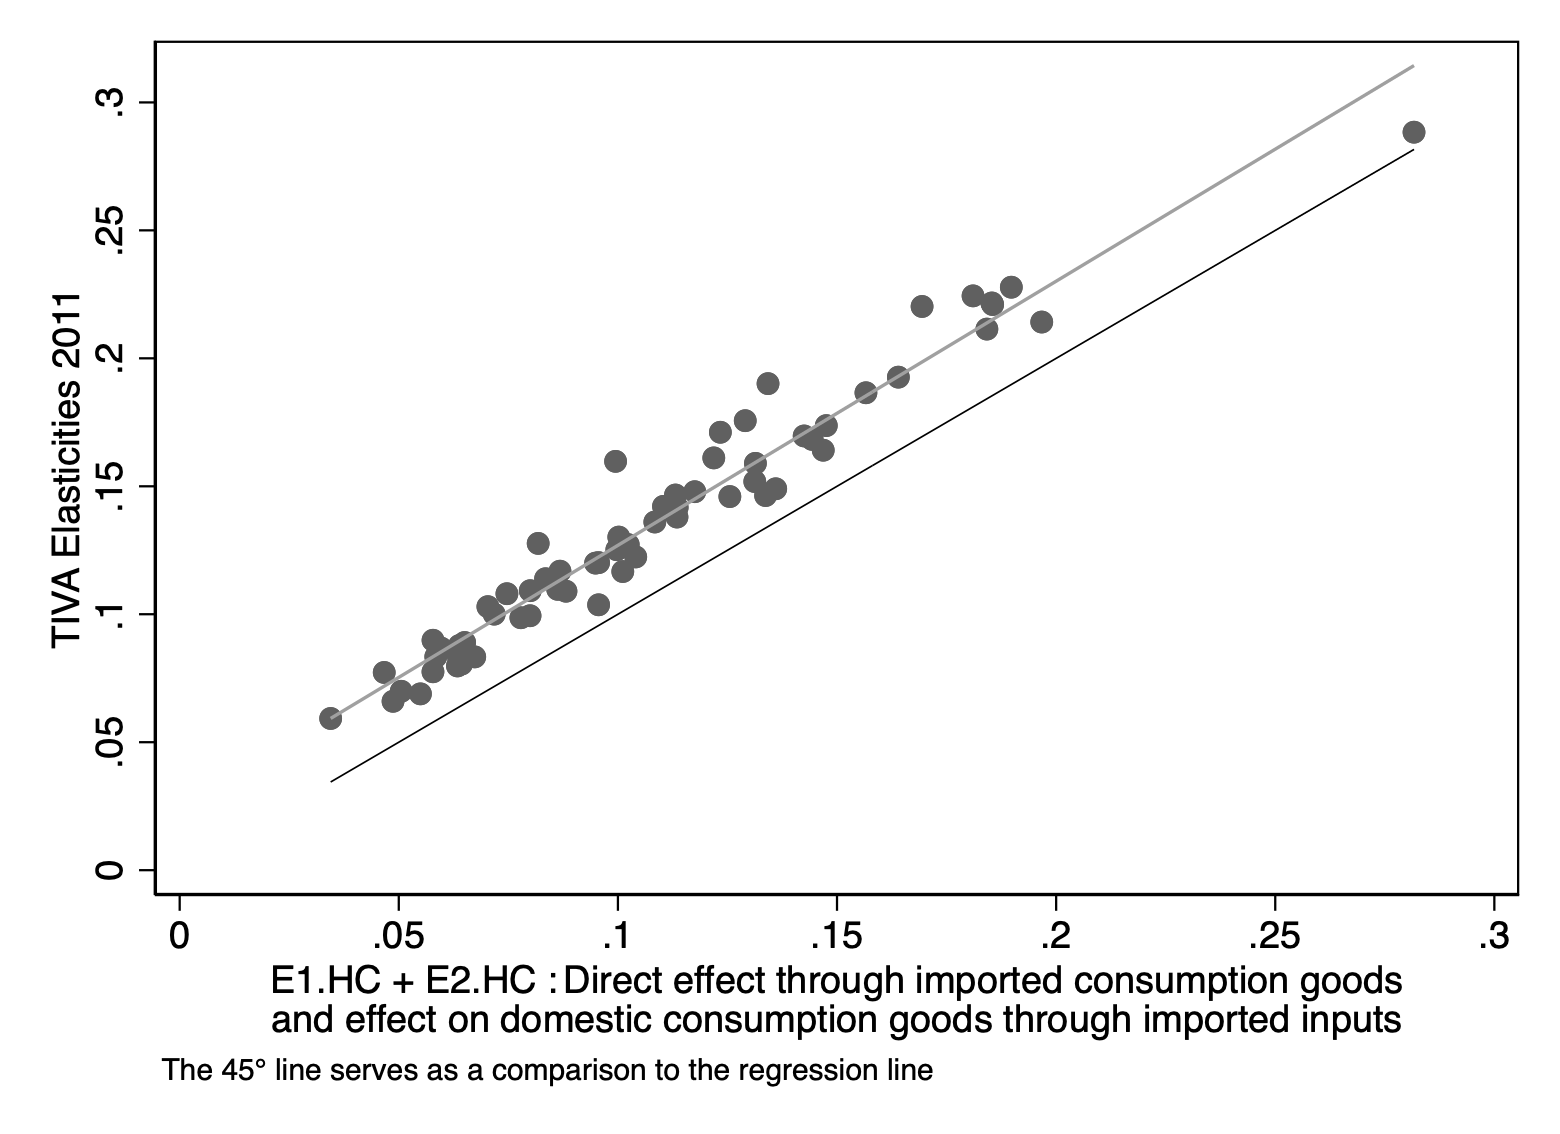
\includegraphics[width=5.0in, height=3.5in]{Comp_s_E1HCE2HC_2011_TIVA_HC.png}\\
	\end{tabular}
	\label{fig:ratiodir_TiVA}
	\floatfoot{Sources: TIVA rev. 3 and authors’ calculations}.
\end{figure}

\begin{figure}[H]
	\centering
	\caption{\footnotesize{\textbf{Evolution of $\alpha$, $\beta$ and $R2$ (TIVA rev. 3)}}}
	\begin{tabular}{c}
		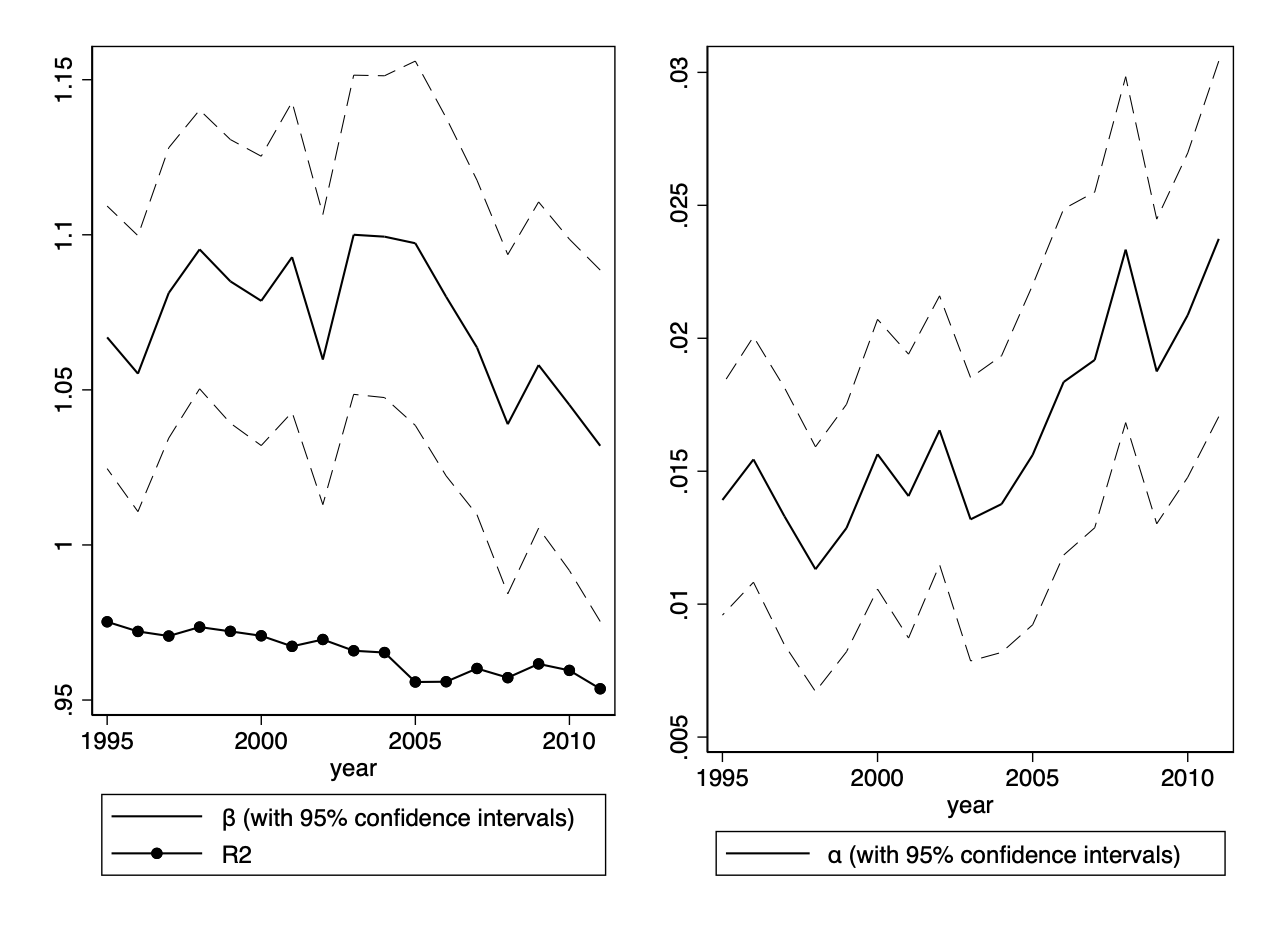
\includegraphics[width=5.0in, height=3.5in]{coef_TIVA_HC}\\
	\end{tabular}
	\label{fig:evolution_coef_TiVA}
	\floatfoot{Sources: TIVA rev. 3 and authors’ calculations}.
\end{figure}

\begin{figure}[H]
	\centering
	\caption{\footnotesize{\textbf{Comparison between $\overline{s}_{i}^{i,HC}$ and $E1.HC^{i,imp}+E2.HC^{i,dom}$ (TIVA rev. 4)}}}
	\begin{tabular}{c}
		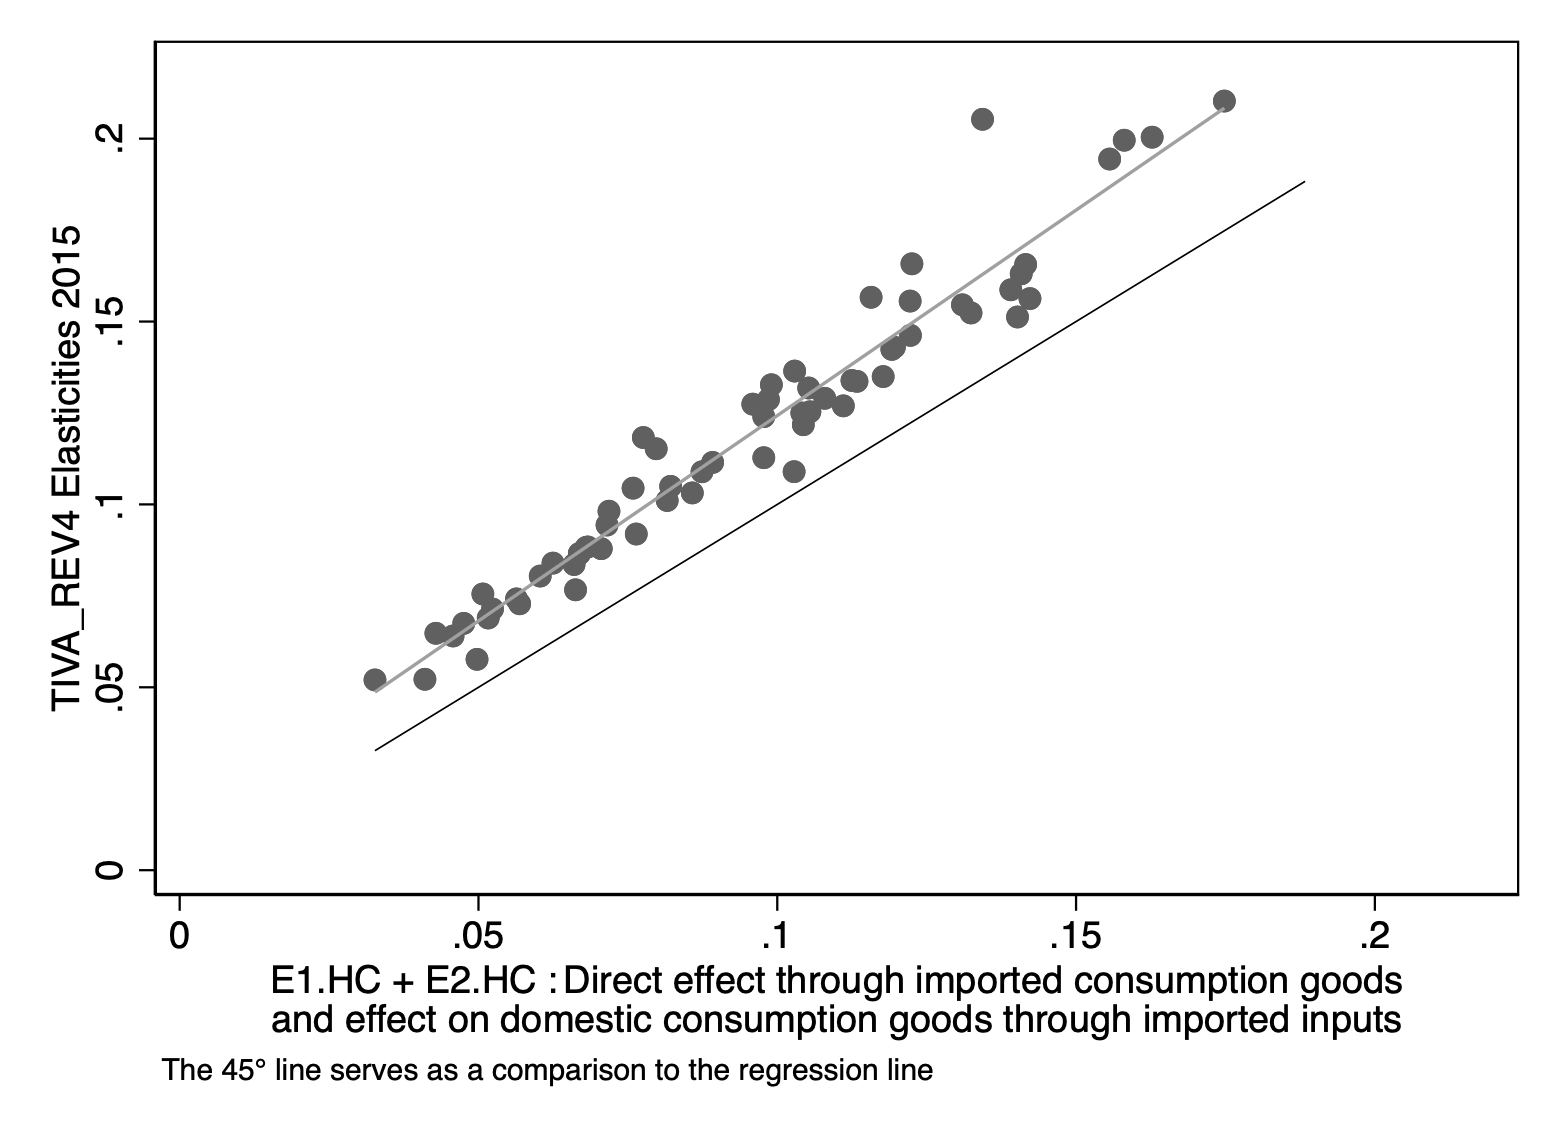
\includegraphics[width=5.0in, height=3.5in]{Comp_s_E1HCE2HC_2015_TIVA_REV4_HC.png}\\
	\end{tabular}
	\label{fig:ratiodir_TiVA_REV4}
	\floatfoot{Sources: TIVA rev. 4 and authors’ calculations}.
\end{figure}

\begin{figure}[H]
	\centering
	\caption{\footnotesize{\textbf{Evolution of $\alpha$, $\beta$ and $R2$ (TIVA rev. 4)}}}
	\begin{tabular}{c}
		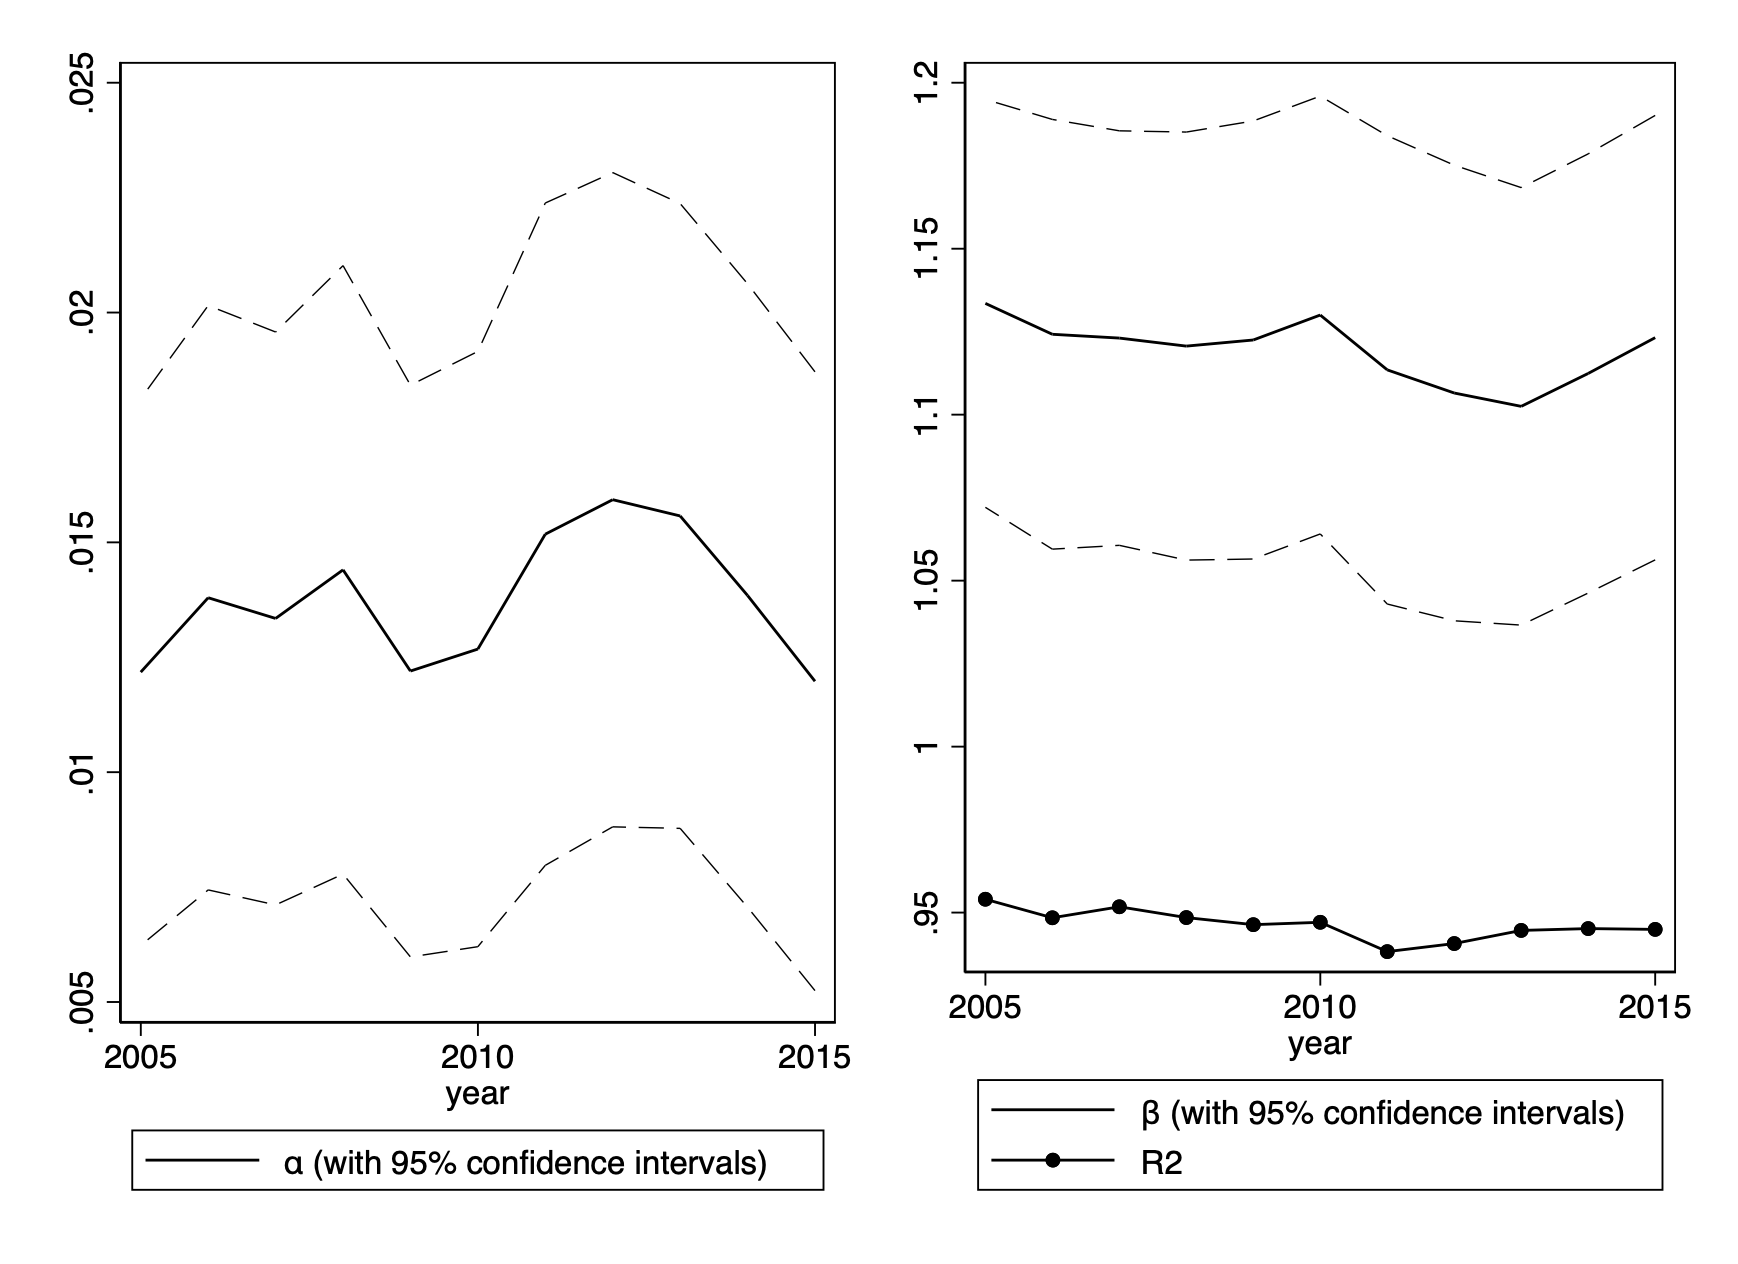
\includegraphics[width=5.0in, height=3.5in]{coef_TIVA_REV4_HC}\\
	\end{tabular}
	\label{fig:evolution_coef_TiVA_REV4}
	\floatfoot{Sources: TIVA rev. 4 and authors’ calculations}.
\end{figure}


\newpage
\section*{Appendix F: Extrapolating the HCE deflator elasticity using household consumption, intermediate consumption and trade statistics}  % je n'avais pas propose un titre plus clair dans une precedent version?
Section 4.2 shows that the sum of the share of imported goods in household consumption and the share of imported inputs in household consumption of domestic goods ($E1.HC + E2.HC$) is a good predictor of the HCE deflator elasticity to the exchange rate. 
However, these data ($E1.HC$ and $E2.HC$) are not up-to-date for a large number of countries, as they are not routinely computed by national statistical institutes. 
Section 4.3 shows that trade and GDP data are a good predictor of the HCE deflator elasticity.
In this appendix, we perform an intermediate exercise.
As in section 4.3, we identify consumption and intermediary goods imports using the CEPII BACI database and the BEC classification.
In contrast to section 4.3, we relate these imports to household consumption and intermediate consumption instead of the GDP.
While the World Bank provides regular estimates for household consumption, estimates for intermediate consumptions are lacking. 
Eurostat provides estimates for intermediate consumption for European countries.
%VF comme la source n'est pas précisee je mets en commentaire \footnote{And some others for selected years Eurostat, BEC -- PRÉCISER LA SOURCE}. 
Combining these three data sources (BACI, World Bank and Eurostat), we compute the share of imported consumption goods in household consumption and the share of imported inputs in all inputs. 
%%We mimick equation 16 in the main text by equation \ref{eq:eq8}. 
%We estimate successive cross-sections of equation \ref{eq:eq8} to check whether the proxy is reliable. 
%
%\begin{equation}
%	\begin{array}{llll}
%		\overline{s}_{i}^{i,HC}= \alpha &+  \beta_1  \frac{\textnormal{imported consumption goods}_i}{\textnormal{household consumption}_i} \\ & +  \beta_2  \left[    \frac{\textnormal{imported intermediate goods}_i}{\textnormal{intermediate consumption}_i}*\frac{\textnormal{domestic consumption goods}_i}{\textnormal{household consumption}_i}\right] +\varepsilon_i 
%	\end{array} 
%	\label{eq:eq8}
%\end{equation}
%
%Figure \ref{fig:evolution_b_reg2} mirrors Figure 13 in the main text. 
%The results are less promising: the $R^2$ is smaller and declining over time, and the estimated coefficient is not constant.
%
%
%\begin{figure}[H]
%	\centering
%	\caption{\footnotesize{\textbf{Evolution of $\beta$ and $R2$ (WIOD) using Eurostat data to approximate E1.HC + E2.HC (limited number of countries)}}}
%	\begin{tabular}{c}
%		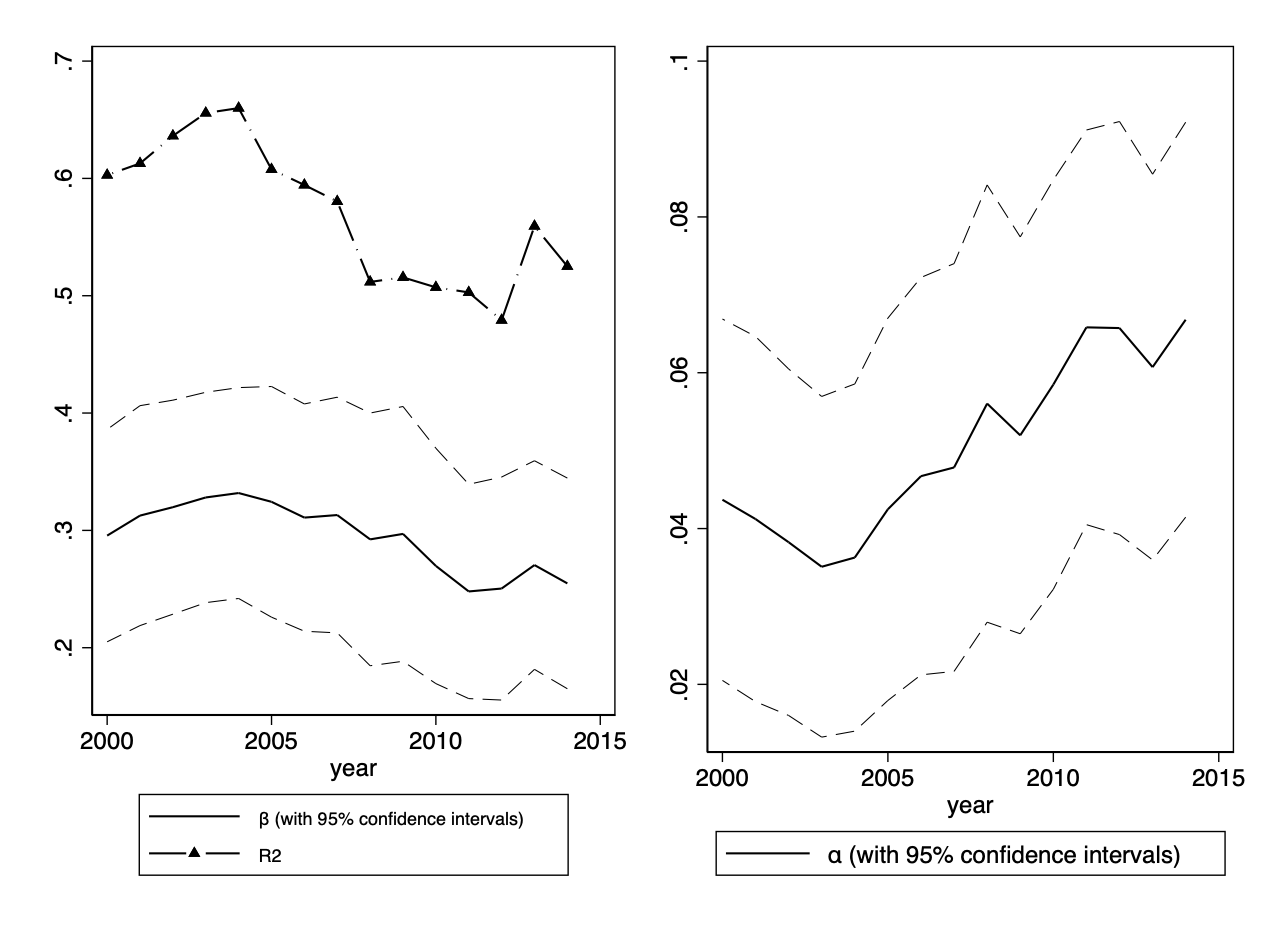
\includegraphics[width=5.0in, height=3.5in]{reg2_WIOD.png}\\
%	\end{tabular}
%	\label{fig:evolution_b_reg2}
%	\floatfoot{Sources: WIOD and authors’ calculations}
%\end{figure}
%
%%pas facile à comprendre, je propose de reformuler
%%Estimating successive cross-sections of equation \ref{eq:eq8} is a demanding test. 
%%In addition, cross-sections do not take advantage of country-specific information.
%%To address this issue, we run a panel regression with country-fixed effects.
%%We assume that $\beta$ is constant over time for each country $i$ (equation \ref{eq:eq9}).
%Estimating successive cross-sections of equation \ref{eq:eq8} is a demanding test. 
%In addition, these regressions fail to account for country-specific determinants of the HCE deflator elasticity.
%A less demanding test consists in running

We then run a panel regression with country fixed-effects, assuming that the coefficients are constant over time and explain within-country variations. 
To take into account year-specific effects, we add two year-specific variables, i.e. the GDP-weighted mean of each variable of interest (see equation \ref{eq:eq9}). 


\begin{equation}
	\begin{array}{llll}
		\overline{s}_{i,t}^{i,t,HC}= \alpha &+  \beta_1  \frac{\textnormal{imported consumption goods}_{i,t}}{\textnormal{household consumption}_{i,t}} \\
		& + \beta_2 \left[ \frac{\textnormal{imported intermediate goods}_{i,t}}{\textnormal{intermediate consumption}_{i,t}}*\frac{\textnormal{domestic consumption goods}_{i,t}}{\textnormal{houshold consumption}_{i,t}}\right] \\ 
		&+  \beta_3 \frac{\textnormal{Total imported consumption goods}_t}{\textnormal{Total household consumption}_t} \\
		& + \beta_4  \left[ \frac{\textnormal{Total imported intermediate goods}_t}{\textnormal{Total intermediate consumption}_t}*\frac{\textnormal{Total domestic consumption goods}_t}{\textnormal{Total household consumption}_t} \right] \\ 
		& +fe_{i}+\varepsilon_{i,t}
	\end{array}
	\label{eq:eq9}
\end{equation}

We run the panel regressions for the period 2000 to 2008 and estimate out-of-sample elasticities for each country $i$ for 2014. 
The outcome is close to the elasticity computed with WIOD for 2014, despite a slight downward bias (see Figure \ref{fig:panel_pred1}).

\begin{figure}[H]
	\centering
	\caption{\footnotesize{\textbf{Comparing the HCE deflator elasticity in 2014 (WIOD) and the prediction from a panel regression on the 2000-2008 period with fixed effects}}}
	\begin{tabular}{c}
		\includegraphics[width=5.0in, height=3.5in]{"resultats_reg2_doigt_mouille_WIOD_pred_6y_trend_no".png}\\
	\end{tabular}
	\label{fig:panel_pred1}
\end{figure}



\newpage
\section*{Appendix E: Transmission channels of an exchange rate variation in the two-country, one-sector case}\label{AnalyticalAppendix}
%je retire car cést tres bizare ce titre de sous section, j'ai cru que cétait une erreur
%\subsection*{The issue}

As a reminder from the paper, where $\overline{s}_{i}^{i,HC}$ corresponds to the impact of an exchange rate variation on consumer prices:  
\begin{equation}
\begin{array}{lccl}
\overline{s}_{i}^{i,HC}&=S^i.HC^i=E1.HC^i+E2.HC^i+E3.HC^i+E4.HC^i \\
&=E1.HC^{i,imp}+E2.HC^{i,dom}+E3.HC^{i,imp}+E4.HC^i
\end{array} 
\end{equation}

and

\begin{equation}
\begin{array}{lccl}
S^ i&=&C^i	&+ \left(\hat{C}^i_\$.{\cal B}^i+{C^i}{\tilde{{\cal B}^i}}\right)*{{(I-{\cal A})}^{-1}} \\
S^i &=&\underbrace{C^i}_{\substack{\text{(E1) direct effect through} \\ \text{ imported consumption goods}}}&+ \underbrace{{C^i}{\tilde{{\cal B}^i}}}_{\substack{\text{(E2) effect on} \\ \text{ \emph{domestic} consumption goods} \\ \text{ through \emph{imported} inputs}}}  + \underbrace{\hat{C}^i_\$.{\cal B}^i}_{\substack{\text{(E3)  effect on} \\ \text{\emph{imported} consumption goods} \\ \text{through \emph{domestic} inputs}}} \\ &&+\underbrace {\left( \hat{C}^i_\$.{\cal B}^i + {C^i}{\tilde{{\cal B}^i}}\right)*{{(I-{\cal A})}^{-1}}*{\cal A}}_{\text{(E4) residual}} \\
\end{array}
\end{equation}



When the domestic currency appreciates, $E1$ and $E2$ reduce country $i$'s consumer prices, whereas $E3$ increases them. $E1$ and $E2$ are easy to compute with national input-output matrices, whereas world input-output matrices are needed for computing $E3$ and $E4$.

Unexpectedly, $E3.HC + E4.HC$ does not vary much with the openness rate of the economy (see Figure 12 of the main text).


Let us focus on the two-country, one-sector economy: 

\begin{gather*}
E1=C=\left(0,-c\right)
\\
E2=C.\tilde{\cal B}^i=\left(0,-c\right).\left(\begin{matrix}0&0\\a_{2,1}&0\end{matrix}\right)=\left(-c.a_{2,1},0\right)
\\
E3=(c,0).\left(\begin{matrix}0&a_{1,2}\\0&0\end{matrix}\right)=\left(0,c.a_{1,2}\right)
\end{gather*}

\begin{gather*}
E1.HC = \left(0,-c\right).\left(\begin{matrix}1-f\\f\end{matrix}\right)=-f.c
\\
E2.HC=\left(-c.a_{2,1},0\right).\left(\begin{matrix}1-f\\f\end{matrix}\right)=-c.a_{2,1}.\left(1-f\right)
\\ 
E3.HC=\left(0,c.a_{1,2}\right).\left(\begin{matrix}1-f\\f\end{matrix}\right)=f.c.a_{1,2}
\end{gather*}

We do not lose any generality by normalising the shock $c$ to 1. 

And :
\begin{gather}
\bar{s}-E1.HC-E2.HC=\left(\begin{array}{r}
-\frac{a_{12} a_{21}^{2} - a_{11} a_{21} a_{22} + {\left(a_{11} - a_{12}\right)} a_{21} - {\left(a_{12} a_{21}^{2} - a_{11} a_{21} a_{22} - {\left(a_{11} - 1\right)} a_{12} + {\left(a_{11} - 2 \, a_{12}\right)} a_{21}\right)} f}{a_{12} a_{21} - {\left(a_{11} - 1\right)} a_{22} + a_{11} - 1}
\end{array}\right)
\end{gather}
We assume that:
$\frac{a_{1,1}}{a_{2,1}}=\frac{1-f}{f}$ and $a_{1,1}+a_{2,1}=a$. \\ 
So
$a_{1,1}=(1-f)a$ and $a_{2,1}=fa$. \\

Then:

\begin{gather}
\bar{s}-E1.HC-E2.HC=\left(\begin{array}{r}
-\frac{{\left(a^{2} a_{12} + a^{2} a_{22} - a^{2}\right)} f^{3} - {\left(2 \, a^{2} a_{22} - 2 \, a^{2} + {\left(a^{2} + a\right)} a_{12}\right)} f^{2} + {\left(a^{2} a_{22} - a^{2} + a_{12}\right)} f}{{\left(a - 1\right)} a_{22} - {\left(a a_{12} + a a_{22} - a\right)} f - a + 1}
\end{array}\right)
\end{gather}

The derivative of this according to f is: 
\begin{gather*}
\left(\begin{array}{r}
-\frac{{\left({\left(a^{2} a_{12} + a^{2} a_{22} - a^{2}\right)} f^{3} - {\left(2 \, a^{2} a_{22} - 2 \, a^{2} + {\left(a^{2} + a\right)} a_{12}\right)} f^{2} + {\left(a^{2} a_{22} - a^{2} + a_{12}\right)} f\right)} {\left(a a_{12} + a a_{22} - a\right)}}{{\left({\left(a - 1\right)} a_{22} - {\left(a a_{12} + a a_{22} - a\right)} f - a + 1\right)}^{2}} \\
- \frac{a^{2} a_{22} + 3 \, {\left(a^{2} a_{12} + a^{2} a_{22} - a^{2}\right)} f^{2} - a^{2} - 2 \, {\left(2 \, a^{2} a_{22} - 2 \, a^{2} + {\left(a^{2} + a\right)} a_{12}\right)} f + a_{12}}{{\left(a - 1\right)} a_{22} - {\left(a a_{12} + a a_{22} - a\right)} f - a + 1}
\end{array}\right)
\end{gather*}

The sign of this expression is difficult to study. We hence move to a numerical application.

%\subsection*{Numerical application} 
%inutile dávoir des sections avec des titres enormes pour láppednix, je propose de retirer, la phrasse precedente annonce l'applicationn numeriique
Based on WIOD 2014, we compute the ratio between value added and production, which corresponds to: 
egen total=rowtotal(vAUS1-vROW) and then (161-74)/161=0.54.

To simplify, we assume that the ratio is equal to 0.5.
\begin{gather*}
a_{1,1}+a_{1,2}=a_{2,1}+a_{2,2}=0.5 \\
\frac{a_{1,2}}{a_{1,1}+a_{1,2}}=f \\
a_{2,1}=0.48 \\
a_{2,2}=0.02
\end{gather*}
In that case:

\begin{gather*}
\begin{array}{r}
\bar{s}-E1.HC-E2.HC = \frac{-0.125 \, f^{3} + 0.245 \, f^{2} - 0.11 \, f}{-0.25 \, f - 0.26
}
\end{array}
\end{gather*}

Which yields Figures \ref{fig:resid} and \ref{fig:tous_les_E}.
\begin{figure}[H]
	\begin{center}
		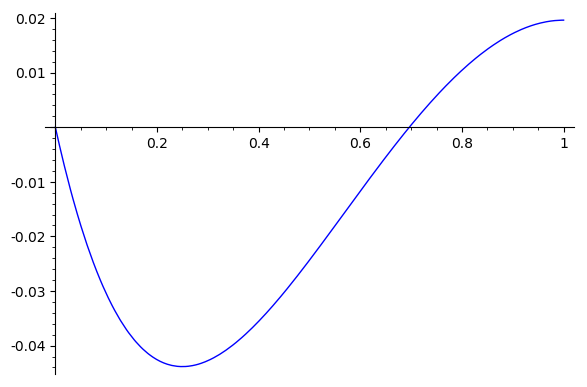
\includegraphics{etude_residu.png}
		\caption{$\bar{s}-E1.HC-E2.HC$ as a function of the openness rate}
		\label{fig:resid}
	\end{center}
\end{figure}

Actual openness rates in the sample vary between 0.15 and 0.50. In that range, the relationship between the openness rate and the residual is not monotonous (see Figure \ref{fig:resid}).

Figure \ref{fig:tous_les_E} confirms that, in that numerical exercise, the total effect is dominated by the direct effect through imported consumption goods and, to a lesser extent, the effect on domestic consumption goods through imported inputs. 
The other effects are approximately additive if the openness rate ranges from 0.15 to 0.50.

\begin{figure}[H]
	\begin{center}
		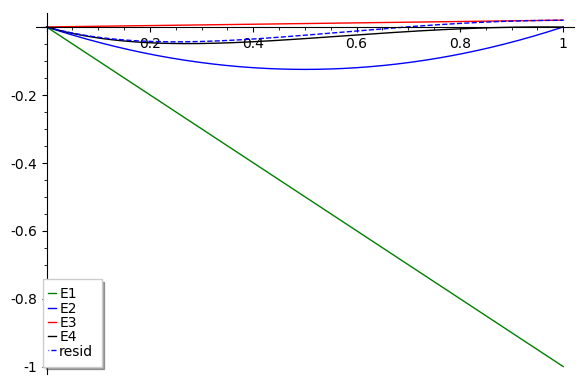
\includegraphics{etude_tous_les_E.png}
		\caption{E1.HC, E2.HC, E3.HC, E4.HC and the "residual"  ($\bar{s}-E1.HC-E2.HC$) as a function of the openness rate}
		\label{fig:tous_les_E}
	\end{center}
\end{figure}



\end{document}
